\section{Theorie}
% Es sollen die wichtigsten theoretischen Formeln und Zusammenh�nge einmal ausf�hrlich erkl�rt werden
Die wichtigsten theoretischen Grundlagen f�r den Versuch sollen zusammengefasst werden.
\subsection{Michelson Interferometer}
Der schematische Aufbau f�r die Verwendung des Michelson Interferometers ist in Abbildung \ref{fig:schem_auf} dargestellt.
\begin{figure}[H]
\centering
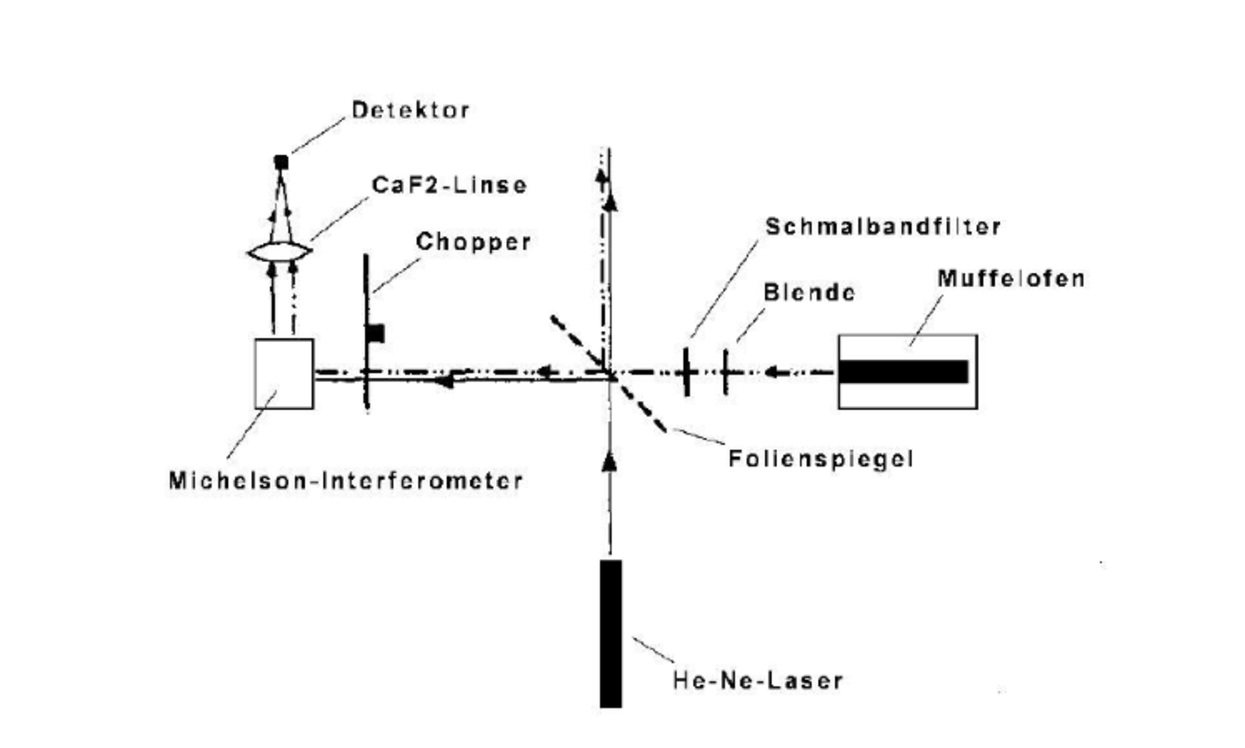
\includegraphics[scale = 1,trim = 3cm 0cm 3cm 0cm]{Schematischer_Aufbau_Michelson}
\caption{Aufbau des Experimentes \cite{Schematischer_Aufbau}}
\label{fig:schem_auf}
\end{figure}
Der Strahlengang im Michelson Interferometer ist in Abbildung \ref{fig:strahlengang} zu sehen.
\begin{figure}[H]
\centering
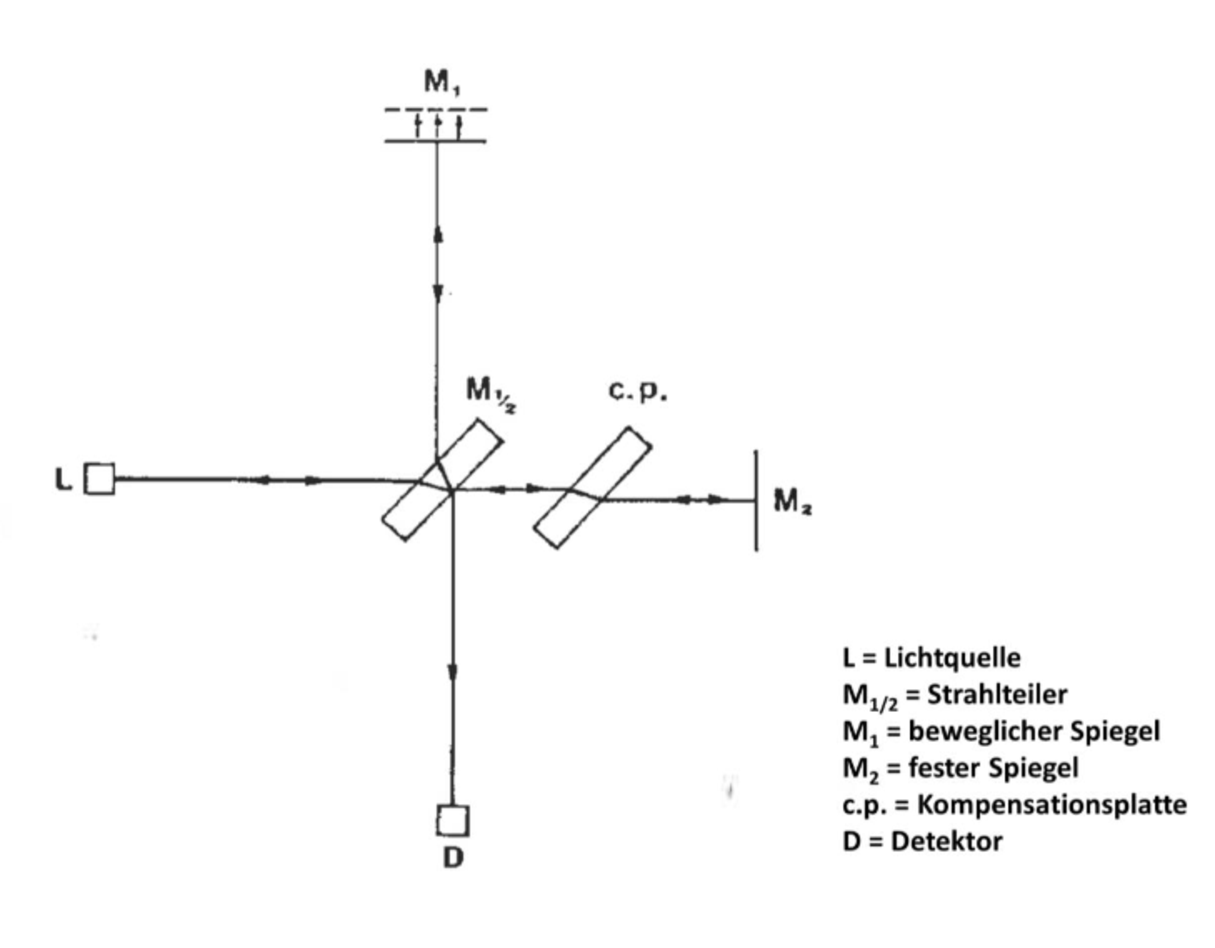
\includegraphics[scale = 0.8,trim = 3cm 0cm 3cm 0cm]{Strahlengang_Michelson}
\caption{Strahlengang im Michelson Interferometer \cite{Schematischer_Aufbau}}
\label{fig:strahlengang}
\end{figure}
"`Innerhalb des Interferometers wird die einfallende Strahlung an der R�ckseite des ZnSe-Strahlteilers auf den beweglichen Spiegel reflektiert, der �ber einen Hebelmechanismus von einem Getriebemotor angetrieben wird. Der Hebelmechanismus ist mit einer Mikrometerschraube versehen und �bertr�gt den Vorschub des Antriebssystems in einem Verh�ltnis von ca. 5:1 auf den Spiegel. Mikrometerschraube und Getriebemotor sind �ber eine Achse miteinander verbunden, auf der ein Drehgeber befestigt ist, der die Messwertaufnahme des verwendeten LabView-Programms steuert. Die zum festen Interferometerspiegel durch die ZnSe-Strahlteilerplatte und eine ZnSe-Kompensationsplatte transmittierte Strahlung interferiert nach Reflexion am Spiegel an der strahlteilenden Schicht mit dem vom beweglichen Spiegel reflektierten Strahlungsanteil und wird mit einer CaF2 -Linse auf eine pyroelektrischen Detektor fokussiert."' (Zitat \cite{Schematischer_Aufbau} Seite 2, Kapitel 4 Messaufbau Zeile 8ff.)
Die Bedingung f�r konstruktive bzw. destruktive Interferenz ergibt sich aus dem Gangunterschied, welcher durch die Verschiebung des beweglichen Spiegels eingestellt werden kann. Das Licht durchl�uft den Gangunterschied $\delta_l$ zweimal, sodass sich die Beziehungen \ref{eqn:konstr_interfer} und \ref{eqn:destr_interfer} f�r konstruktive bzw. destruktive Interferenz ergeben.
\begin{align}
n\lambda = 2\delta_l \hspace{0.1cm},\hspace{0.2cm} n \in \mathbb{N}_0
\label{eqn:konstr_interfer}
\\
\left(n+\frac{1}{2}\right)\lambda = 2\delta_l \hspace{0.1cm},\hspace{0.2cm} n \in \mathbb{N}_0
\label{eqn:destr_interfer}
\end{align}
Bei der Bestimmung von $\delta_l$ muss die �bersetzung der Mikrometerschraube beachtet werden.
\subsection{Strahlungsintensit�t}
Der Zusammenhang zwischen der Intensit�t $I$ und $\delta_l$ kann \cite{Staatsex_Michels} entnommen werden. F�r monochromatische Strahlung ergibt sich Gleichung \ref{eqn:monochr}.
\begin{align}
I(\delta_l) = \frac{I(1/\lambda)}{2}\left(1+\cos\left(\frac{2\pi \delta_l}{\lambda}\right)\right)
\label{eqn:monochr}
\end{align}
Unter Vernachl�ssigung des konstanten Offsets, sowie unter Ber�cksichtigung von Strahlungsverlusten erh�lt man daraus Gleichung \ref{eqn:monochr2}.
\begin{align}
I(\delta_l) = B(1/\lambda)\cos\left(\frac{2\pi \delta_l}{\lambda}\right)
\label{eqn:monochr2}
\end{align}
Nach Integration �ber alle Wellenzahlen (1/$\lambda$) (Gleichung \ref{eqn:polychr}) erh�lt man die Intensit�t von polychromatischem Licht $I_{poly}$ in Abh�ngigkeit des Gangunterschiedes.
\begin{align}
I(\delta_l)_{poly} = \int_0^\infty d(1/\lambda) B(1/\lambda)\cos\left(\frac{2\pi \delta_l}{\lambda}\right)
\label{eqn:polychr}
\end{align}
Aus der Fourierr�cktransformation kann dann $B(\lambda)$ nach Gleichung \ref{eqn:poly_r�ck} bestimmt werden.
\begin{align}
B(1/\lambda) = 2 \int_0^\infty d\delta_l I(\delta_l)_{poly}\cos\left(\frac{2\pi \delta_l}{\lambda}\right)
\label{eqn:poly_r�ck}
\end{align}
Als Ansatz f�r die sp�tere Analyse des Interferogramms mit Schmalbandfilter kann f�r $B(1/\lambda)$ eine Gaussfunktion verwendet werden. F�r I wird dabei eine modulierte Gaussfunktion angenommen. Es ergibt sich die in Gleichung \ref{eqn:B_schmalband} beschriebene Beziehung, wobei $b = 1/\lambda_{max}$ die Wellenzahl maximaler Transmission ist und $4/a$ die $1/e$-Breite des Filters ist.
\begin{align}
B(1/\lambda) = \frac{a}{2\sqrt{\pi}}\exp\left(-\frac{(a2\pi(b-1/\lambda))^2}{4}\right)
\label{eqn:B_schmalband}
\end{align}